\begin{figure}[H]
  \centering
  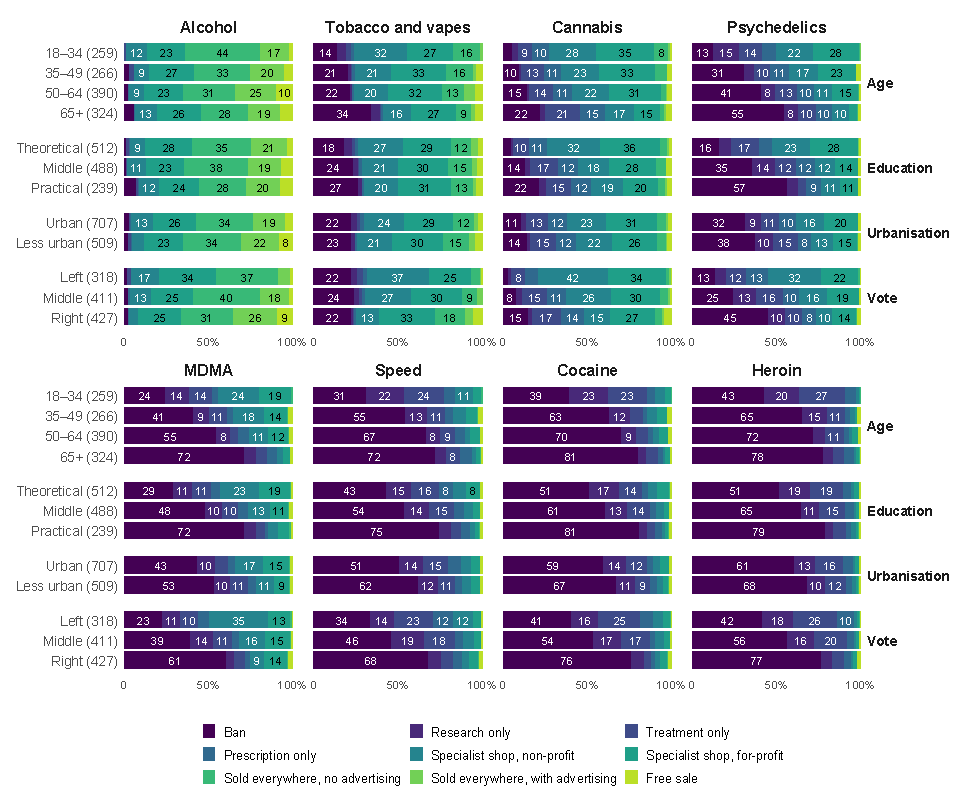
\includegraphics[width=\linewidth]{out/fig_gradient_grid.pdf}
  \caption{Preferred regulatory model per substance by age, education, urbanisation and vote. Each bar shows the weighted shares of a group choosing each of the nine options, from ban (left) to free sale (right); colours as in Figure~\ref{fig:policy_preferences}, labels from 8\%. Numbers in brackets are respondents (unweighted). Urban = very high or high address density, less urban = moderate, low or none (23 respondents without urbanisation are not in those rows). Vote (TK 2025) by the party's general left-right position in the Chapel Hill Expert Survey 2024 \parencite{rovny2025}, split into equal thirds of the 0--10 scale: left = SP, PvdD, GroenLinks-PvdA; middle = DENK, Volt, CU, D66, 50PLUS (2019 score), CDA; right = VVD, BBB, SGP, PVV, FvD and JA21 (not rated; placed between VVD and PVV). Other parties, blank and non-voters ($n = 83$) are not in the vote rows.}
  \label{fig:gradient}
\end{figure}
